% Apuntes de la fase final de la práctica: lo que NO está en apuntes/ (invarianzas, síntesis, comparativa,
% estadística por dataset, conceptos de computación evolutiva, ablaciones, coste).
% Compilar desde esta carpeta:  latexmk -pdf apuntes_final.tex
% Las cifras salen de ../numeros.tex y ../tablas.tex (generados por ../analisis.py); figuras de ../figuras/.
\documentclass[apuntes]{uc3mmaster}

\titulo{Transformación evolutiva de atributos: invarianzas, síntesis y evaluación rigurosa}
\subtitulo{Apuntes de la fase final de la práctica}
\asignatura{IA con inspiración biológica}
\tipo{Apuntes}
\autor{Andrea López Salazar}{}

\usepackage{tikz}
\usetikzlibrary{babel,arrows.meta,positioning,calc,shapes.geometric,decorations.pathreplacing,fit}
\usepackage{pgfplots}
\pgfplotsset{compat=1.18}
\usepackage{booktabs}
\usepackage{multirow}
\graphicspath{{../figuras/}}
% Generado por analisis.py: NO editar a mano.
\newcommand{\nDatasets}{12}
\newcommand{\nParticiones}{5}
\newcommand{\nCasos}{60}
\newcommand{\relRL}{0{,}96}
\newcommand{\cambioRL}{$-$4{,}4\,\%}
\newcommand{\casosRL}{36/60}
\newcommand{\dsRL}{7/12}
\newcommand{\pRL}{$1{,}000$}
\newcommand{\cambioVsEstRL}{$-$2{,}6\,\%}
\newcommand{\dsVsEstRL}{6/12}
\newcommand{\pVsEstRL}{$1{,}000$}
\newcommand{\peorDsRL}{$+$20{,}9\,\%}
\newcommand{\relKNN}{0{,}76}
\newcommand{\cambioKNN}{$-$24{,}3\,\%}
\newcommand{\casosKNN}{56/60}
\newcommand{\dsKNN}{12/12}
\newcommand{\pKNN}{$0{,}004$}
\newcommand{\cambioVsEstKNN}{$-$13{,}6\,\%}
\newcommand{\dsVsEstKNN}{10/12}
\newcommand{\pVsEstKNN}{$0{,}048$}
\newcommand{\peorDsKNN}{$-$0{,}4\,\%}
\newcommand{\relArbol}{1{,}00}
\newcommand{\cambioArbol}{$+$0{,}1\,\%}
\newcommand{\casosArbol}{34/60}
\newcommand{\dsArbol}{7/12}
\newcommand{\pArbol}{$1{,}000$}
\newcommand{\cambioVsEstArbol}{$+$0{,}1\,\%}
\newcommand{\dsVsEstArbol}{7/12}
\newcommand{\pVsEstArbol}{$1{,}000$}
\newcommand{\peorDsArbol}{$+$5{,}0\,\%}
\newcommand{\relRF}{1{,}00}
\newcommand{\cambioRF}{$+$0{,}5\,\%}
\newcommand{\casosRF}{27/60}
\newcommand{\dsRF}{5/12}
\newcommand{\pRF}{$1{,}000$}
\newcommand{\cambioVsEstRF}{$+$0{,}5\,\%}
\newcommand{\dsVsEstRF}{5/12}
\newcommand{\pVsEstRF}{$1{,}000$}
\newcommand{\peorDsRF}{$+$4{,}1\,\%}
\newcommand{\cambioSintRL}{$-$1{,}3\,\%}
\newcommand{\pSintRL}{$0{,}705$}
\newcommand{\dsSintRL}{7/12}
\newcommand{\relSintRL}{0{,}99}
\newcommand{\cambioSintKNN}{$-$0{,}3\,\%}
\newcommand{\pSintKNN}{$0{,}705$}
\newcommand{\dsSintKNN}{7/12}
\newcommand{\relSintKNN}{1{,}00}
\newcommand{\cambioSintArbol}{$+$0{,}3\,\%}
\newcommand{\pSintArbol}{$1{,}000$}
\newcommand{\dsSintArbol}{7/12}
\newcommand{\relSintArbol}{1{,}00}
\newcommand{\cambioSintRF}{$-$0{,}1\,\%}
\newcommand{\pSintRF}{$1{,}000$}
\newcommand{\dsSintRF}{7/12}
\newcommand{\relSintRF}{1{,}00}
\newcommand{\cambioRedRL}{$+$1{,}8\,\%}
\newcommand{\pRedRL}{$0{,}380$}
\newcommand{\dsRedRL}{5/12}
\newcommand{\relRedRL}{1{,}02}
\newcommand{\cambioRedKNN}{$+$1{,}0\,\%}
\newcommand{\pRedKNN}{$0{,}330$}
\newcommand{\dsRedKNN}{4/12}
\newcommand{\relRedKNN}{1{,}01}
\newcommand{\cambioRedArbol}{$+$1{,}4\,\%}
\newcommand{\pRedArbol}{$0{,}330$}
\newcommand{\dsRedArbol}{3/12}
\newcommand{\relRedArbol}{1{,}01}
\newcommand{\cambioRedRF}{$+$2{,}8\,\%}
\newcommand{\pRedRF}{$0{,}049$}
\newcommand{\dsRedRF}{1/12}
\newcommand{\relRedRF}{1{,}03}
\newcommand{\dimMedia}{83\,\%}
\newcommand{\fracEliminados}{22\,\%}
\newcommand{\dimMin}{38\,\%}
\newcommand{\dimMax}{92\,\%}
\newcommand{\mMedia}{0{,}4}
\newcommand{\fracConSintesis}{25\,\%}
\newcommand{\tauMediana}{0{,}18}
\newcommand{\casosNmenosUno}{38/60}
\newcommand{\wLat}{2{,}91}
\newcommand{\wLon}{2{,}85}
\newcommand{\wPop}{0{,}03}
\newcommand{\wInc}{0{,}41}
\newcommand{\fracApagados}{10\,\%}
\newcommand{\nCompCasos}{60}
\newcommand{\compMLKRRL}{$-$1{,}8\,\%}
\newcommand{\compMLKRKNN}{$-$22{,}5\,\%}
\newcommand{\compMLKRArbol}{$+$2{,}0\,\%}
\newcommand{\compMLKRRF}{$+$2{,}6\,\%}
\newcommand{\rangoMLKR}{5{,}7}
\newcommand{\compPGRL}{$-$15{,}7\,\%}
\newcommand{\compPGKNN}{$-$18{,}0\,\%}
\newcommand{\compPGArbol}{$+$0{,}7\,\%}
\newcommand{\compPGRF}{$+$0{,}8\,\%}
\newcommand{\rangoPG}{4{,}6}
\newcommand{\compYJMVRL}{$+$2{,}4\,\%}
\newcommand{\compYJMVKNN}{$-$14{,}5\,\%}
\newcommand{\compYJMVArbol}{$+$1{,}5\,\%}
\newcommand{\compYJMVRF}{$+$1{,}7\,\%}
\newcommand{\rangoYJMV}{5{,}0}
\newcommand{\compCuantRL}{$+$8{,}1\,\%}
\newcommand{\compCuantKNN}{$-$11{,}8\,\%}
\newcommand{\compCuantArbol}{$+$0{,}1\,\%}
\newcommand{\compCuantRF}{$+$0{,}0\,\%}
\newcommand{\rangoCuant}{6{,}4}
\newcommand{\compEstPCARL}{$-$1{,}8\,\%}
\newcommand{\compEstPCAKNN}{$-$12{,}4\,\%}
\newcommand{\compEstPCAArbol}{$-$0{,}6\,\%}
\newcommand{\compEstPCARF}{$-$1{,}9\,\%}
\newcommand{\rangoEstPCA}{4{,}6}
\newcommand{\compPCAnoventaRL}{$+$0{,}6\,\%}
\newcommand{\compPCAnoventaKNN}{$-$10{,}4\,\%}
\newcommand{\compPCAnoventaArbol}{$+$19{,}3\,\%}
\newcommand{\compPCAnoventaRF}{$+$17{,}9\,\%}
\newcommand{\rangoPCAnoventa}{8{,}1}
\newcommand{\compPCAcvRL}{$-$1{,}0\,\%}
\newcommand{\compPCAcvKNN}{$-$12{,}0\,\%}
\newcommand{\compPCAcvArbol}{$+$18{,}7\,\%}
\newcommand{\compPCAcvRF}{$+$15{,}1\,\%}
\newcommand{\rangoPCAcv}{7{,}4}
\newcommand{\compPsrRL}{$-$6{,}1\,\%}
\newcommand{\compPsrKNN}{$-$25{,}0\,\%}
\newcommand{\compPsrArbol}{$-$1{,}1\,\%}
\newcommand{\compPsrRF}{$-$2{,}3\,\%}
\newcommand{\rangoPsr}{3{,}2}
\newcommand{\compPRL}{$-$4{,}4\,\%}
\newcommand{\compPKNN}{$-$24{,}3\,\%}
\newcommand{\compPArbol}{$+$0{,}1\,\%}
\newcommand{\compPRF}{$+$0{,}5\,\%}
\newcommand{\rangoP}{4{,}7}
\newcommand{\mejorAlt}{estándar + PCA}
\newcommand{\rangoMejorAlt}{4{,}6}
\newcommand{\nReps}{10}
\newcommand{\vMedia}{0{,}80}
\newcommand{\vFracUno}{22\,\%}
\newcommand{\nSintMedia}{3{,}9}
\newcommand{\ctrlIniAleat}{$+$0{,}6\,\%}
\newcommand{\pCtrlIniAleat}{$1{,}000$}
\newcommand{\ctrlIniAleatRL}{$+$1{,}7\,\%}
\newcommand{\ctrlSigmaBajo}{$+$0{,}5\,\%}
\newcommand{\pCtrlSigmaBajo}{$1{,}000$}
\newcommand{\ctrlSigmaBajoRL}{$-$0{,}1\,\%}
\newcommand{\ctrlSigmaAlto}{$+$0{,}9\,\%}
\newcommand{\pCtrlSigmaAlto}{$1{,}000$}
\newcommand{\ctrlSigmaAltoRL}{$-$0{,}4\,\%}
\newcommand{\ctrlPobDoble}{$+$0{,}2\,\%}
\newcommand{\pCtrlPobDoble}{$1{,}000$}
\newcommand{\ctrlPobDobleRL}{$-$0{,}2\,\%}
\newcommand{\nAblCasos}{24}
\newcommand{\ctrlPesos}{$+$2{,}2\,\%}
\newcommand{\ctrlPesosRL}{$+$6{,}5\,\%}
\newcommand{\pCtrlPesos}{$0{,}424$}
\newcommand{\ctrlExp}{$+$10{,}0\,\%}
\newcommand{\ctrlExpRL}{$+$2{,}2\,\%}
\newcommand{\pCtrlExp}{$0{,}012$}
\newcommand{\ctrlAleat}{$+$6{,}2\,\%}
\newcommand{\ctrlAleatRL}{$+$3{,}0\,\%}
\newcommand{\pCtrlAleat}{$0{,}012$}
\newcommand{\ctrlMI}{$+$14{,}9\,\%}
\newcommand{\ctrlMIRL}{$+$6{,}8\,\%}
\newcommand{\pCtrlMI}{$0{,}012$}
\newcommand{\ctrlYJMI}{$+$11{,}0\,\%}
\newcommand{\ctrlYJMIRL}{$+$10{,}3\,\%}
\newcommand{\pCtrlYJMI}{$0{,}014$}
\newcommand{\nCtrlCasos}{24}
\newcommand{\rangoCeroR}{$+$2{,}2\,\%}
\newcommand{\pRangoCero}{$1{,}000$}
\newcommand{\dsPeorRangoCero}{7}
\newcommand{\rangoUnoR}{$+$0{,}3\,\%}
\newcommand{\pRangoUno}{$1{,}000$}
\newcommand{\dsPeorRangoUno}{6}
\newcommand{\rangoCuatroR}{$+$0{,}5\,\%}
\newcommand{\pRangoCuatro}{$1{,}000$}
\newcommand{\dsPeorRangoCuatro}{7}
\newcommand{\rangoOchoR}{$+$1{,}7\,\%}
\newcommand{\pRangoOcho}{$0{,}256$}
\newcommand{\dsPeorRangoOcho}{9}
\newcommand{\bordeUno}{11\,\%}
\newcommand{\bordeDos}{7\,\%}
\newcommand{\bordeCuatro}{8\,\%}
\newcommand{\bordeOcho}{5\,\%}
\newcommand{\nRango}{24}
\newcommand{\mleFueraDos}{24\,\%}
\newcommand{\nAlgCasos}{24}
\newcommand{\rangoCMA}{1{,}9}
\newcommand{\algMejor}{CMA-ES}
\newcommand{\algKNNcma}{$-$25{,}7\,\%}
\newcommand{\algKNNaleat}{$-$21{,}0\,\%}
\newcommand{\algKNNmin}{$-$24{,}8\,\%}
\newcommand{\algKNNmax}{$-$23{,}3\,\%}
\newcommand{\segMediana}{191}
\newcommand{\segMax}{243}
\newcommand{\msPorEval}{191}
\newcommand{\segMLKR}{16{,}8}
\newcommand{\segPG}{6{,}1}
\newcommand{\segYJMV}{0{,}6}
\newcommand{\popMin}{11}
\newcommand{\popMax}{13}
\newcommand{\muMin}{5}
\newcommand{\muMax}{6}
\newcommand{\muEffMin}{3{,}4}
\newcommand{\muEffMax}{4{,}0}
\newcommand{\genMin}{77}
\newcommand{\genMax}{91}
\newcommand{\nParadaPresupuesto}{12}
\newcommand{\nParadaTotal}{12}
\newcommand{\evalMejorMediana}{971}
\newcommand{\evalMejorMin}{658}
\newcommand{\mejoraFitnessMediana}{$-$12{,}1\,\%}
\newcommand{\sigmaFinMin}{0{,}007}
\newcommand{\sigmaFinMax}{0{,}06}
\newcommand{\cribSelRL}{$-$2{,}5\,\%}
\newcommand{\cribSelKNN}{$-$23{,}9\,\%}
\newcommand{\cribSelArbol}{$+$0{,}1\,\%}
\newcommand{\cribSelRF}{$+$0{,}8\,\%}
\newcommand{\cribDimSel}{72\,\%}
\newcommand{\cribFijoRL}{$-$5{,}4\,\%}
\newcommand{\cribFijoKNN}{$-$25{,}0\,\%}
\newcommand{\cribFijoArbol}{$-$0{,}5\,\%}
\newcommand{\cribFijoRF}{$+$0{,}0\,\%}
\newcommand{\cribDimFijo}{89\,\%}
\newcommand{\cribPcaRL}{$-$2{,}7\,\%}
\newcommand{\cribPcaKNN}{$-$23{,}9\,\%}
\newcommand{\cribPcaArbol}{$+$0{,}8\,\%}
\newcommand{\cribPcaRF}{$+$1{,}9\,\%}
\newcommand{\cribDimPca}{70\,\%}
\newcommand{\cribFijoNoReduce}{27/60}
% Generado por analisis.py: filas de las tablas (una macro por tabla).
\newcommand{\filasPrincipal}{%
R. lineal & 0{,}98 & 0{,}94 & \textbf{0{,}96} & 7/12 & $1{,}000$ & $-$2{,}6\,\%\\
KNN & 0{,}88 & 0{,}75 & \textbf{0{,}76} & 12/12 & $0{,}004$ & $-$13{,}6\,\%\\
Árbol & 1{,}00 & 0{,}99 & \textbf{1{,}00} & 7/12 & $1{,}000$ & $+$0{,}1\,\%\\
RF & 1{,}00 & 0{,}98 & \textbf{1{,}00} & 5/12 & $1{,}000$ & $+$0{,}5\,\%\\
}
\newcommand{\filasDimension}{%
diabetes & 10 & 8{,}0 & 0{,}6 & 8{,}6 & 0{,}46\\
concrete & 8 & 6{,}6 & 0{,}0 & 6{,}6 & 0{,}47\\
stock & 9 & 7{,}6 & 0{,}4 & 8{,}0 & 0{,}30\\
space\_ga & 6 & 3{,}8 & 0{,}4 & 4{,}2 & 0{,}09\\
sulfur & 6 & 5{,}0 & 0{,}0 & 5{,}0 & 0{,}01\\
wine\_quality & 11 & 9{,}6 & 0{,}2 & 9{,}8 & 0{,}41\\
kin8nm & 8 & 7{,}0 & 0{,}0 & 7{,}0 & 0{,}34\\
bank8FM & 8 & 6{,}8 & 0{,}2 & 7{,}0 & 0{,}05\\
puma8NH & 8 & 2{,}2 & 2{,}4 & 4{,}6 & 1{,}83\\
house\_8L & 8 & 7{,}0 & 0{,}0 & 7{,}0 & 0{,}12\\
cpu\_small & 12 & 10{,}8 & 0{,}2 & 11{,}0 & 0{,}19\\
california & 8 & 6{,}6 & 0{,}0 & 6{,}6 & 0{,}02\\
}
\newcommand{\filasComparativa}{%
estándar & 0{,}98 & 0{,}88$^*$ & 1{,}00 & 1{,}00 & 5{,}3 & 1{,}00\\
YJ máx.\ verosimilitud & 1{,}02 & 0{,}85$^*$ & 1{,}01 & 1{,}02 & 5{,}0 & 1{,}00\\
cuantiles & 1{,}08 & 0{,}88$^*$ & 1{,}00 & 1{,}00 & 6{,}4 & 1{,}00\\
solo PCA (95\,\%) & 1{,}01 & 0{,}90$^*$ & 1{,}19$^*$ & 1{,}18$^*$ & 8{,}1 & 0{,}79\\
solo PCA (\% por VC) & 0{,}99 & 0{,}88$^*$ & 1{,}19$^*$ & 1{,}15 & 7{,}4 & 0{,}91\\
estándar + su PCA & 0{,}98 & 0{,}88$^*$ & 0{,}99 & 0{,}98 & 4{,}6 & 2{,}00\\
MLKR & 0{,}98 & 0{,}78 & 1{,}02 & 1{,}03 & 5{,}7 & 1{,}00\\
PG (gplearn) & \textbf{0{,}84} & 0{,}82$^*$ & 1{,}01 & 1{,}01 & 4{,}6 & 2{,}00\\
$P$ sin reducir & 0{,}94 & \textbf{0{,}75} & \textbf{0{,}99} & \textbf{0{,}98} & 3{,}2 & 2{,}00\\
\textbf{$P$} & 0{,}96 & 0{,}76 & 1{,}00 & 1{,}00 & 4{,}7 & 0{,}83\\
}
\newcommand{\filasAblacion}{%
\multicolumn{4}{@{}l}{\emph{Piezas}}\\
\quad solo pesos ($\lambda=1$) & $+$2{,}2\,\% & $+$6{,}5\,\% & $-$0{,}1\,\%\\
\quad solo exponentes ($w=1$) & $+$10{,}0\,\%$^*$ & $+$2{,}2\,\% & $+$0{,}4\,\%\\
\midrule
\multicolumn{4}{@{}l}{\emph{Sin búsqueda}}\\
\quad pesos por inf.\ mutua & $+$14{,}9\,\%$^*$ & $+$6{,}8\,\% & $+$3{,}6\,\%\\
\quad YJ (MV) + pesos inf.\ mutua & $+$11{,}0\,\% & $+$10{,}3\,\% & $+$3{,}6\,\%\\
\midrule
\multicolumn{4}{@{}l}{\emph{Búsqueda}}\\
\quad búsqueda aleatoria (1000 puntos) & $+$6{,}2\,\%$^*$ & $+$3{,}0\,\% & $+$2{,}0\,\%\\
\midrule
\multicolumn{4}{@{}l}{\emph{Inicio}}\\
\quad media inicial aleatoria & $+$0{,}6\,\% & $+$1{,}7\,\% & $+$0{,}6\,\%\\
\quad $\sigma_0=0{,}1$ & $+$0{,}5\,\% & $-$0{,}1\,\% & $+$0{,}8\,\%\\
\quad $\sigma_0=0{,}4$ & $+$0{,}9\,\% & $-$0{,}4\,\% & $+$0{,}6\,\%\\
\quad población $\times2$ & $+$0{,}2\,\% & $-$0{,}2\,\% & $+$1{,}3\,\%\\
\midrule
\multicolumn{4}{@{}l}{\emph{Rango}}\\
\quad $\lambda\in[-1,1]$ & $+$0{,}3\,\% & $+$1{,}5\,\% & $-$0{,}3\,\%\\
\quad $\lambda\in[-4,4]$ & $+$0{,}5\,\% & $+$1{,}4\,\% & $+$1{,}1\,\%\\
\quad $\lambda\in[-8,8]$ & $+$1{,}7\,\% & $+$5{,}0\,\% & $+$1{,}4\,\%\\
}
\newcommand{\filasControles}{%
solo pesos ($\lambda=1$) & $+$2{,}2\,\% & $+$6{,}5\,\% & $-$0{,}1\,\%\\
solo exponentes ($w=1$) & $+$10{,}0\,\%$^*$ & $+$2{,}2\,\% & $+$0{,}4\,\%\\
búsqueda aleatoria & $+$6{,}2\,\%$^*$ & $+$3{,}0\,\% & $+$2{,}0\,\%$^*$\\
pesos por inf.\ mutua & $+$14{,}9\,\%$^*$ & $+$6{,}8\,\% & $+$3{,}6\,\%\\
YJ (MV) + pesos inf.\ mutua & $+$11{,}0\,\%$^*$ & $+$10{,}3\,\% & $+$3{,}6\,\%\\
}
\newcommand{\filasAlgoritmos}{%
\textbf{CMA-ES} & 1{,}9 & $-$25{,}7\,\% & $-$7{,}7\,\%\\
AG (propio) & 2{,}8 & $-$24{,}4\,\% & $-$8{,}5\,\%\\
HS & 3{,}2 & $-$24{,}5\,\% & $-$8{,}3\,\%\\
BBO & 4{,}4 & $-$24{,}8\,\% & $-$8{,}0\,\%\\
PSO & 4{,}5 & $-$24{,}1\,\% & $-$5{,}1\,\%\\
DE & 5{,}4 & $-$23{,}3\,\% & $-$5{,}9\,\%\\
ABC & 5{,}9 & $-$24{,}0\,\% & $-$2{,}4\,\%\\
búsqueda aleatoria & 7{,}9 & $-$21{,}0\,\% & $-$4{,}9\,\%\\
}
\newcommand{\filasCoste}{%
P (CMA-ES, 1000 evaluaciones) & 190{,}6 & 242{,}6\\
MLKR & 16{,}8 & 41{,}8\\
PG (gplearn) & 6{,}1 & 14{,}1\\
PCA v-CV & 1{,}0 & 11{,}5\\
YJ máx. verosimilitud & 0{,}6 & 4{,}3\\
cuantiles & 0{,}1 & 0{,}8\\
estándar + PCA & 0{,}0 & 0{,}0\\
}
\newcommand{\filasDatasets}{%
diabetes & 442 & 10\\
concrete & 1\,030 & 8\\
stock & 950 & 9\\
space\_ga & 3\,107 & 6\\
sulfur & 10\,000 & 6\\
wine\_quality & 6\,497 & 11\\
kin8nm & 8\,192 & 8\\
bank8FM & 8\,192 & 8\\
puma8NH & 8\,192 & 8\\
house\_8L & 10\,000 & 8\\
cpu\_small & 8\,192 & 12\\
california & 20\,640 & 8\\
}


\definecolor{azul}{HTML}{2E6DB4}
\definecolor{naranja}{HTML}{D9731A}
\definecolor{verde}{HTML}{2F9467}
\definecolor{rojo}{HTML}{C0392B}
\definecolor{gris}{HTML}{8C8C8C}
\colorlet{azulm}{azul}\colorlet{naranjam}{naranja}\colorlet{verdem}{verde}\colorlet{grism}{gris}

\newtcolorbox{idea}[1][]{uc3mbox,colback=verde!8,colframe=verde,coltitle=verde!70!black,colbacktitle=verde!8,
  title={Idea clave\ifx&#1&\else\ (#1)\fi}}
\newtcolorbox{cuidado}[1][]{uc3mbox,colback=rojo!6,colframe=rojo,coltitle=rojo!80!black,colbacktitle=rojo!6,
  title={Cuidado\ifx&#1&\else\ (#1)\fi}}

\begin{document}
\makeportada
\tableofcontents
\newpage

%=====================================================================================================
\section*{Cómo leer estos apuntes}
\addcontentsline{toc}{section}{Cómo leer estos apuntes}
Estos apuntes continúan los de \texttt{apuntes/}, que ya explican el problema, Yeo-Johnson, los pesos, CMA-ES paso a
paso, el fitness y los primeros experimentos. Aquí está \textbf{lo nuevo de la fase final}: el bloque de síntesis,
por qué funciona (invarianzas), cómo se compara con otras técnicas, cómo evaluar con rigor, los conceptos de
computación evolutiva aplicados a nuestra búsqueda y qué conclusiones cambiaron al endurecer la evaluación.

\begin{figure}[h]\centering
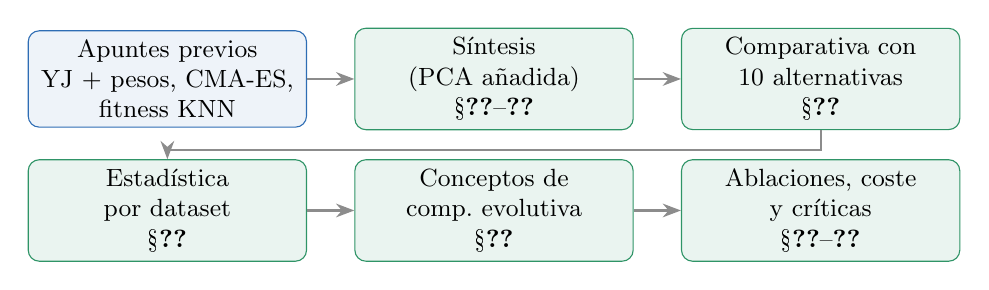
\begin{tikzpicture}[node distance=4mm and 6mm,
  caja/.style={draw=azul, rounded corners, fill=azul!8, align=center, text width=3.3cm, font=\small, minimum height=1.2cm},
  nueva/.style={caja, draw=verde, fill=verde!10},
  fl/.style={-{Stealth}, thick, gris}]
\node[caja] (a) {Apuntes previos\\YJ + pesos, CMA-ES,\\fitness KNN};
\node[nueva, right=of a] (b) {Síntesis\\(PCA añadida)\\\S\ref{sec:invarianzas}--\ref{sec:sintesis}};
\node[nueva, right=of b] (c) {Comparativa con\\10 alternativas\\\S\ref{sec:comparativa}};
\node[nueva, below=of a] (d) {Estadística\\por dataset\\\S\ref{sec:estadistica}};
\node[nueva, right=of d] (e) {Conceptos de\\comp.\ evolutiva\\\S\ref{sec:evolutiva}};
\node[nueva, right=of e] (f) {Ablaciones, coste\\y críticas\\\S\ref{sec:ablacion}--\ref{sec:criticas}};
\draw[fl] (a)--(b); \draw[fl] (b)--(c); \draw[fl] (c.south) -- ++(0,-0.25) -| (d.north);
\draw[fl] (d)--(e); \draw[fl] (e)--(f);
\end{tikzpicture}
\caption{Mapa de lo nuevo. En verde, lo que no está en los apuntes anteriores.}
\end{figure}

\begin{resultado}[El método final en una frase]
$P$ aprende con CMA-ES, solo con el entrenamiento, $X'=[\,z\mid V^\top(z-\bar z)\,]$, donde
$z_j=w_j\,(\psi(x_j;\lambda_j)-\mu_j)/\sigma_j$ (\emph{forma} + \emph{relevancia}) y $V^\top(z-\bar z)$ son las
componentes principales del espacio aprendido (\emph{síntesis}).
\end{resultado}

%=====================================================================================================
\section{Invarianzas: qué ``ve'' cada modelo}\label{sec:invarianzas}
El enunciado exige mejorar un modelo \emph{arbitrario}. La pregunta útil no es ``¿qué transformación es mejor?'',
sino ``¿qué transformaciones \emph{no puede notar} cada modelo?''. Si un modelo es indiferente a una transformación,
esa transformación no le puede ayudar ni perjudicar.

\begin{definicion}[Invarianza]
Un modelo $M$ es \textbf{invariante} a una transformación $T$ si entrenarlo y evaluarlo con $T(X)$ da exactamente
las mismas predicciones que con $X$: $M_{T(X_t)}(T(x))=M_{X_t}(x)$ para todo $x$.
\end{definicion}

\subsection{KNN: invariante a isometrías y a escalados globales}
\begin{proposicion}
Si $T(x)=c\,Qx+b$ con $Q$ ortogonal ($Q^\top Q=I$), $c>0$ y $b$ un vector, KNN es invariante a $T$.
\end{proposicion}
\textit{Demostración.} $\lVert T(x)-T(x')\rVert=c\,\lVert Q(x-x')\rVert=c\,\lVert x-x'\rVert$. Todas las distancias se
multiplican por la misma constante, así que el orden de vecinos no cambia y la media de sus $y$ tampoco. $\square$

Rotar, trasladar o escalar \emph{todo} por igual no cambia KNN. Lo que sí le cambia es escalar \emph{cada atributo
por separado} (los pesos) o deformarlo de forma no lineal (Yeo-Johnson).

\subsection{Regresión lineal: invariante a transformaciones afines invertibles}
\begin{proposicion}
Si $T(x)=Ax+b$ con $A$ invertible, la regresión lineal por mínimos cuadrados es invariante a $T$. Más en general,
solo importa el \emph{espacio columna} de la matriz de diseño $[\mathbf 1, X]$.
\end{proposicion}
\textit{Demostración.} El ajuste por mínimos cuadrados es la proyección ortogonal de $y$ sobre el espacio columna de
$[\mathbf 1,X]$. Con $T$, la matriz pasa a $[\mathbf 1, XA^\top+\mathbf 1b^\top]$, que genera el mismo espacio. Misma
proyección, mismas predicciones. $\square$

A la regresión lineal solo le cambian las transformaciones \textbf{no lineales} por atributo (Yeo-Johnson). Los pesos
$w_j$ son un escalado lineal, así que \emph{por sí solos} no le afectan (aunque sí le llegan indirectamente porque
se aprenden junto con los $\lambda$).

\subsection{Árboles: invariantes a transformaciones monótonas por atributo}
\begin{proposicion}
Si $T(x)=(\phi_1(x_1),\dots,\phi_n(x_n))$ con cada $\phi_j$ estrictamente creciente, un árbol encuentra las mismas
particiones del entrenamiento.
\end{proposicion}
\textit{Idea.} Un corte ``$x_j\le t$'' separa los puntos según su orden en el atributo $j$, y $\phi_j$ no cambia el
orden. Para cada corte en $X$ existe uno equivalente en $T(X)$. (Ya estaba en los apuntes previos.)

\begin{cuidado}[la invarianza es exacta en entrenamiento, aproximada en test]
El árbol coloca el umbral en el \emph{punto medio} entre dos valores consecutivos del entrenamiento. Tras una
$\phi_j$ no lineal, el punto medio en el espacio transformado no es la imagen del punto medio original, así que un
punto de test que cae \emph{entre} esos dos valores puede ir a la otra rama. Por eso Yeo-Johnson por máxima
verosimilitud cambia un poco a Random Forest (\compYJMVRF) aunque sea monótona, y $P$ sin síntesis da 0,999 y no 1.
Los cuantiles, que también son monótonos, salen exactamente en 1,00.
\end{cuidado}

\subsection{Consecuencia de diseño}
\begin{table}[h]\centering\small
\caption{Qué transformaciones nota cada familia de modelos.}
\begin{tabular}{@{}lccc@{}}\toprule
Transformación & KNN & Regresión lineal & Árbol / RF\\\midrule
Rotación, traslación, escala global & no & no & \textbf{sí} (cambia los ejes)\\
Escala por atributo ($w_j$) & \textbf{sí} & no & no\\
Monótona no lineal por atributo (YJ) & \textbf{sí} & \textbf{sí} & no (aprox.)\\
Añadir combinaciones lineales ortogonales & no & no & \textbf{sí}\\\bottomrule
\end{tabular}
\end{table}

\begin{idea}
Construir $X'$ \textbf{por bloques}, cada uno pensado para lo que una familia puede aprovechar y \textbf{neutro} para
las demás. La última fila de la tabla es exactamente el bloque de síntesis: ayuda a los árboles y, por construcción,
no puede tocar a KNN ni a la regresión lineal.
\end{idea}

%=====================================================================================================
\section{El bloque de síntesis}\label{sec:sintesis}
\subsection{Definición y propiedad}
Sea $Z_t$ el entrenamiento ya transformado por forma y relevancia, $\bar z$ su media y $V$ la matriz de vectores
singulares derechos de $Z_t-\bar z$ (las direcciones principales). La síntesis añade
\[
X' = \big[\,z \;\big|\; p\,\big],\qquad p = V^\top (z-\bar z).
\]
\begin{proposicion}[Síntesis sin coste]
(a) $\lVert[z,p]-[z',p']\rVert^2 = 2\lVert z-z'\rVert^2$: KNN obtiene los mismos vecinos. (b) $p$ es combinación
lineal de $z$ y de la constante: la regresión lineal da las mismas predicciones.
\end{proposicion}
\textit{Demostración.} (a) $p-p'=V^\top(z-z')$ y $V$ es ortogonal, así que $\lVert p-p'\rVert=\lVert z-z'\rVert$; la
distancia al cuadrado es la suma de ambas partes. (b) Por la proposición de la regresión lineal. $\square$

Lo comprobamos numéricamente en el notebook: distancias exactamente $\times2$, predicciones de KNN idénticas y de la
regresión lineal iguales hasta $10^{-13}$.

\subsection{Por qué ayuda a un árbol: cortes oblicuos}
\begin{figure}[h]\centering
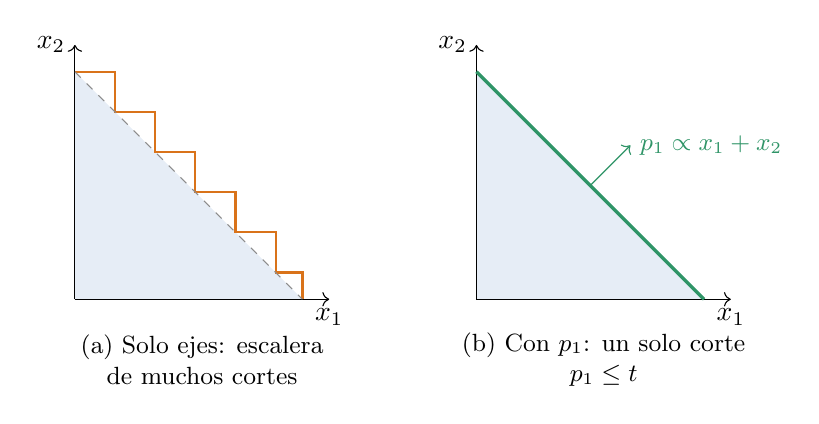
\begin{tikzpicture}[scale=0.85]
\begin{scope}
\fill[azul!12] (0,0) -- (3.4,0) -- (0,3.4) -- cycle;
\draw[->] (0,0) -- (3.8,0) node[below] {$x_1$}; \draw[->] (0,0) -- (0,3.8) node[left] {$x_2$};
\draw[naranja, thick] (0,3.4) -- (0.6,3.4) -- (0.6,2.8) -- (1.2,2.8) -- (1.2,2.2) -- (1.8,2.2) -- (1.8,1.6)
      -- (2.4,1.6) -- (2.4,1.0) -- (3.0,1.0) -- (3.0,0.4) -- (3.4,0.4) -- (3.4,0);
\draw[gris, dashed] (0,3.4) -- (3.4,0);
\node[align=center, font=\small] at (1.9,-0.9) {(a) Solo ejes: escalera\\de muchos cortes};
\end{scope}
\begin{scope}[xshift=6cm]
\fill[azul!12] (0,0) -- (3.4,0) -- (0,3.4) -- cycle;
\draw[->] (0,0) -- (3.8,0) node[below] {$x_1$}; \draw[->] (0,0) -- (0,3.8) node[left] {$x_2$};
\draw[verde, very thick] (0,3.4) -- (3.4,0);
\draw[->, verde] (1.7,1.7) -- (2.3,2.3) node[right, font=\small] {$p_1\propto x_1+x_2$};
\node[align=center, font=\small] at (1.9,-0.9) {(b) Con $p_1$: un solo corte\\$p_1\le t$};
\end{scope}
\end{tikzpicture}
\caption{Si la frontera real es diagonal, un árbol con cortes paralelos a los ejes necesita una escalera de muchos
cortes (a). Si se le da la componente $p_1$, la frontera es un solo corte (b).}
\end{figure}

\subsection{Por qué \emph{añadir} y no \emph{sustituir} (``solo PCA'')}
Sustituir $X$ por sus componentes rota los ejes: el árbol gana los oblicuos pero \emph{pierde los originales}, que
en datos reales suelen ser los buenos cortes (``renta $\le 5$''). Añadir conserva los dos. Es la misma idea que
Rotation Forest (Rodríguez et al., 2006), que construye cada árbol sobre componentes principales de subconjuntos de
atributos.

\begin{figure}[h]\centering
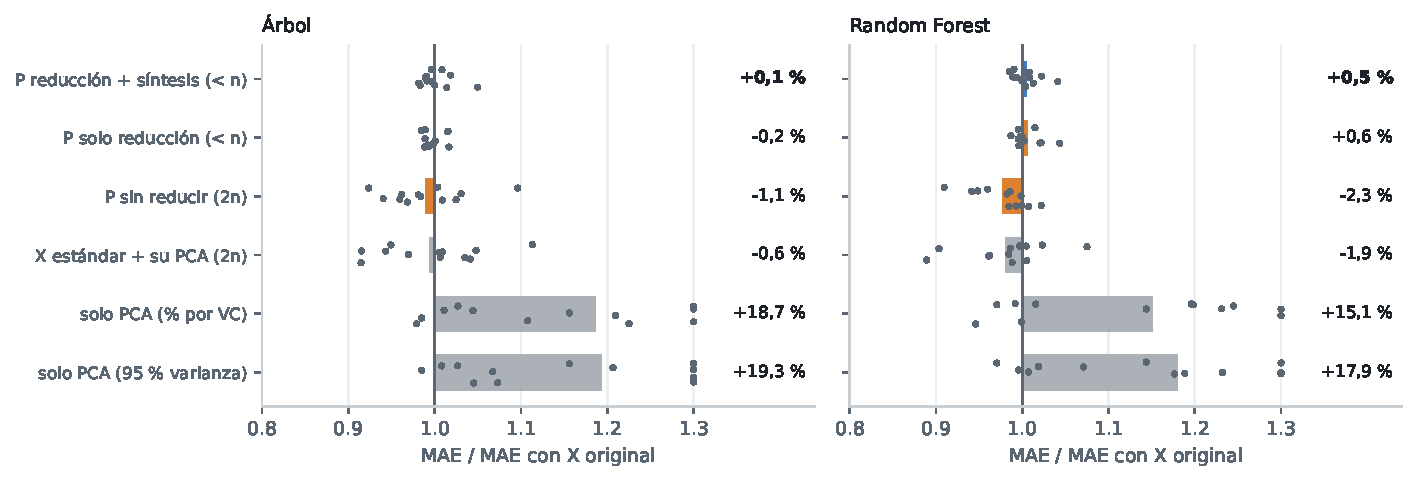
\includegraphics[width=\textwidth]{sintesis}
\caption{Variantes de síntesis en las mismas 60 particiones (punto = dataset, barra = media geométrica).}
\label{fig:sintesis}
\end{figure}

\subsection{Variantes probadas (y por qué se descartaron)}
\begin{table}[h]\centering\small\setlength{\tabcolsep}{4pt}
\caption{Variantes del bloque de síntesis. Cambio del MAE de Random Forest frente a $X$. Las tres primeras
filas son exploratorias (otras particiones); las demás, confirmatorias (Fig.~\ref{fig:sintesis}).}
\begin{tabular}{@{}p{5.6cm}rp{6.2cm}@{}}\toprule
Variante & RF & Por qué se descarta\\\midrule
Elegir componentes con CMA-ES y fitness de árboles & $-2{,}8$\,\% & no gana a añadirlas todas; más parámetros\\
\quad + YJ y pesos con ese fitness & $-3{,}7$\,\% & \textbf{estropea KNN} ($+6{,}2$\,\%)\\
Añadir la predicción de KNN fuera de pliegue & $-3{,}1$\,\% & ayuda mucho en unos datasets y perjudica en otros\\
Solo PCA (95\,\% de varianza) & \compPCAnoventaRF & pierde los ejes originales\\
Solo PCA (\% por validación cruzada) & \compPCAcvRF & ídem\\
$X$ estandarizado + su PCA & \compEstPCARF & casi igual que $P$ (ver idea clave)\\
$P$ con el \% de varianza aprendido por CMA-ES & \compPvRF & peor que añadir todas\\
\textbf{$P$ (todas las componentes)} & \textbf{\compPRF} & elegida: sin parámetros, neutra para KNN y RL\\\bottomrule
\end{tabular}
\end{table}

\begin{definicion}[Predicción fuera de pliegue (\emph{stacking})]
Para cada fila del entrenamiento, se predice $y$ con un modelo entrenado sin ella (validación cruzada) y esa
predicción se añade como atributo. En test se usa el modelo entrenado con todo. Así el atributo no contiene la
propia $y$ de la fila (no hay fuga), pero sí ``lo que sabe KNN''.
\end{definicion}

\textbf{¿Cuántas componentes?} Probamos a que CMA-ES aprenda además $v\in[0{,}5,1]$, la fracción de varianza que
deben cubrir las componentes añadidas. Elige de media $v=\vMedia$ (\nSintMedia{} componentes), pero empeora a RF
(\compPvRF{} frente a \compPRF). La razón: con una síntesis \emph{parcial} ya no se cumple la propiedad (a), las
distancias de KNN cambian y la búsqueda (que optimiza KNN) usa $v$ para reponderar distancias, no para ayudar a los
árboles.

\begin{idea}[lo que de verdad aporta la síntesis]
Con las componentes de $X$ estandarizado, RF mejora \compEstPCARF; con las del espacio aprendido, \compPRF. La
diferencia no es significativa: \textbf{la mejora en árboles viene sobre todo de añadir direcciones oblicuas}, y la
métrica aprendida aporta poco más. Es un resultado honesto que hay que decir así.
\end{idea}

%=====================================================================================================
\section{Comparativa con otras transformaciones}\label{sec:comparativa}
\subsection{Fichas de las alternativas}
\begin{definicion}[Yeo-Johnson por máxima verosimilitud (\texttt{PowerTransformer})]
Elige cada $\lambda_j$ para que el atributo transformado sea lo más \emph{normal} posible:
$\hat\lambda=\arg\max_\lambda\;-\tfrac N2\ln\hat\sigma^2_\lambda+(\lambda-1)\sum_i\mathrm{sign}(x_i)\ln(|x_i|+1)$,
y después estandariza. No mira $y$.
\end{definicion}
\begin{definicion}[Cuantiles (\texttt{QuantileTransformer})]
$x\mapsto\Phi^{-1}(\hat F(x))$: cada atributo pasa por su función de distribución empírica y luego por la inversa de
la normal. Es monótona (los árboles no la notan) y elimina por completo las colas.
\end{definicion}
\begin{definicion}[MLKR, \emph{Metric Learning for Kernel Regression} (Weinberger y Tesauro, 2007)]
Aprende una matriz $A$ y usa $\lVert A(x-x')\rVert$ como distancia. Minimiza por gradiente el error cuadrático
\emph{dejando uno fuera} de la regresión por núcleo
$\hat y_i=\sum_{j\ne i}y_jk_{ij}/\sum_{j\ne i}k_{ij}$, con $k_{ij}=e^{-\lVert A(x_i-x_j)\rVert^2}$. Es el
competidor natural de los pesos: una métrica \emph{completa} ($n^2$ parámetros) frente a la nuestra diagonal
($n$ pesos), pero sin corregir la forma.
\end{definicion}
\begin{definicion}[Construcción de atributos con programación genética (\texttt{gplearn})]
Evoluciona árboles de expresión (con $+,-,\times,\div,\sqrt{\cdot},\log,|\cdot|$) cuya aptitud es la correlación con
$y$; selección por torneo, cruce de subárboles y varias mutaciones, con una penalización por tamaño (parsimonia).
Se quedan los $n$ mejores programas poco correlacionados entre sí y se añaden a $X$. Es la técnica evolutiva
``clásica'' de síntesis de atributos.
\end{definicion}

\subsection{Resultado}
\begin{table}[h]\centering\small\setlength{\tabcolsep}{5pt}
\caption{$e'/e$ por modelo (negrita: mejor; $^*$: $P$ mejor con $p<0{,}05$, Wilcoxon por dataset con Holm) y rango
medio de Friedman (1 = mejor), 60 particiones.}
\begin{tabular}{@{}lccccc@{}}\toprule
Transformación & R.\ lin. & KNN & Árbol & RF & Rango\\\midrule
\filasComparativa\bottomrule
\end{tabular}
\end{table}

\begin{itemize}
\item \textbf{$P$ tiene el mejor rango medio} (\rangoP) y es la única que no empeora a ningún modelo en media.
\item \textbf{No domina en cada modelo.} KNN: MLKR la iguala (\compMLKRKNN{} frente a \compPKNN). Regresión lineal:
gana la programación genética (\compPGRL{} frente a \compPRL), porque construir atributos \emph{no lineales} es
justo lo que necesita un modelo lineal. Random Forest: añadir la PCA de $X$ casi la iguala.
\item \textbf{Normalidad $\neq$ predicción.} Yeo-Johnson por máxima verosimilitud mejora a KNN (\compYJMVKNN) pero
empeora a la regresión lineal (\compYJMVRL). Y los cuantiles, que eliminan las colas, también (\compCuantRL).
\end{itemize}

\begin{idea}
Ninguna transformación gana en todos los modelos: cada una ayuda a la familia cuyo ``punto débil'' corrige. El
argumento de $P$ es ser la mejor \emph{de media} y no perjudicar a ninguna, no ser la mejor en cada una.
\end{idea}

%=====================================================================================================
\section{Diseño experimental y estadística}\label{sec:estadistica}
\subsection{Explorar y confirmar en dos fases}
\begin{figure}[h]\centering
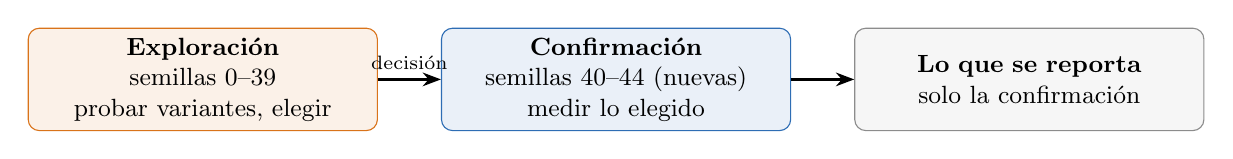
\begin{tikzpicture}[node distance=5mm and 8mm,
  caja/.style={draw, rounded corners, align=center, text width=4.2cm, font=\small, minimum height=1.3cm}]
\node[caja, draw=naranja, fill=naranja!10] (e) {\textbf{Exploración}\\semillas 0--39\\probar variantes, elegir};
\node[caja, draw=azul, fill=azul!10, right=of e] (c) {\textbf{Confirmación}\\semillas 40--44 (nuevas)\\medir lo elegido};
\node[caja, draw=gris, fill=gris!8, right=of c] (r) {\textbf{Lo que se reporta}\\solo la confirmación};
\draw[-{Stealth}, thick] (e) -- node[above, font=\scriptsize] {decisión} (c);
\draw[-{Stealth}, thick] (c) -- (r);
\end{tikzpicture}
\caption{Las particiones que sirven para \emph{elegir} no pueden servir para \emph{medir}: elegir el mejor de muchos
candidatos ruidosos infla su resultado (maldición del ganador).}
\end{figure}

Ejemplos de conclusiones que \textbf{cambiaron} al confirmar con más rigor:
\begin{itemize}
\item PCA con pesos dentro de la búsqueda para KNN: mejoraba en los 12 datasets con 3 particiones, y con 10 nuevas
el efecto desapareció ($-0{,}4$\,\%, $p\approx1$).
\item Rango de $\lambda$: con 500 evaluaciones y contraste por casos, $[-8,8]$ salía $+3{,}1$\,\% ($p<0{,}001$); con
1000 evaluaciones y contraste por dataset, \rangoOchoR{} ($p=$\pRangoOcho).
\item Significación del método: por casos, $p<0{,}001$ en tres modelos; por dataset con Holm, solo KNN.
\end{itemize}

\subsection{La métrica: cociente y media geométrica}
Comparamos con $r=e'/e$ ($r<1$ mejora). Para agregar no se usa la media aritmética: un cociente de $0{,}5$ (la mitad
de error) y uno de $2$ (el doble) deberían compensarse, y la media aritmética da $1{,}25$. La \textbf{media
geométrica} $\exp\big(\tfrac1N\sum\ln r_i\big)$ da $1$: trabaja en escala logarítmica, donde mejorar y empeorar en la
misma proporción son simétricos. Además hace comparables datasets con escalas de $y$ muy distintas.

\subsection{Pseudo-replicación: la unidad es el dataset}
\begin{definicion}[Pseudo-replicación]
Tratar como independientes observaciones que no lo son, lo que infla artificialmente el tamaño muestral y hace
salir significativo lo que no lo es.
\end{definicion}
Las 5 particiones de un mismo dataset comparten la mayoría de sus filas (cada fila está en el entrenamiento del
$\sim$70\,\% de ellas): no son 60 observaciones independientes. La unidad correcta es el \textbf{dataset} ($n=12$):
se resume cada dataset con la media geométrica de sus particiones y se contrasta sobre esos 12 valores
(Demšar, 2006).

\subsection{Wilcoxon de rangos con signo}
Para dos métodos, con $d_i=\ln r_i$ en cada dataset: se ordenan los $|d_i|$, se suman los rangos de los positivos
y de los negativos, y se compara con lo esperable si el signo fuera al azar. No supone normalidad y pesa más las
diferencias grandes que un simple conteo de signos. Con $n=12$ hay $2^{12}=4096$ combinaciones de signos, así que el
$p$ bilateral más pequeño posible es $2/4096\approx0{,}0005$: con pocos datasets, el contraste tiene un suelo.

\subsection{Comparaciones múltiples: Holm}
Si se hacen $m$ contrastes al 5\,\%, la probabilidad de algún falso positivo crece mucho. \textbf{Holm} la controla:
\begin{enumerate}
\item Ordenar los $p$ de menor a mayor: $p_{(1)}\le\dots\le p_{(m)}$.
\item Ajustar $\tilde p_{(i)}=\max_{k\le i}\min\big(1,(m-k+1)\,p_{(k)}\big)$.
\item Rechazar donde $\tilde p<0{,}05$.
\end{enumerate}
\begin{ejemplo}
Con $p=(0{,}0005;\,0{,}027;\,0{,}043;\,0{,}20)$ y $m=4$: $\tilde p=(0{,}002;\,0{,}081;\,0{,}086;\,0{,}20)$. Solo el
primero sobrevive. Es lo que pasa con nuestros cuatro modelos: KNN sale, regresión lineal y RF no.
\end{ejemplo}

\subsection{Muchos métodos: Friedman y Nemenyi}
Para comparar $k$ métodos en $N$ datasets: en cada dataset se ordenan los métodos (rango 1 = mejor) y se promedian
los rangos $\bar R_j$. \textbf{Friedman} contrasta si todos los rangos medios podrían ser iguales. Si se rechaza,
\textbf{Nemenyi} dice qué pares difieren: dos métodos son distinguibles si sus rangos medios se separan más que la
\textbf{diferencia crítica}
\[
CD=q_\alpha\sqrt{\frac{k(k+1)}{6N}},\qquad k=11,\;N=12,\;q_{0{,}05}\approx3{,}22\;\Rightarrow\;CD\approx4{,}36.
\]
\begin{figure}[h]\centering
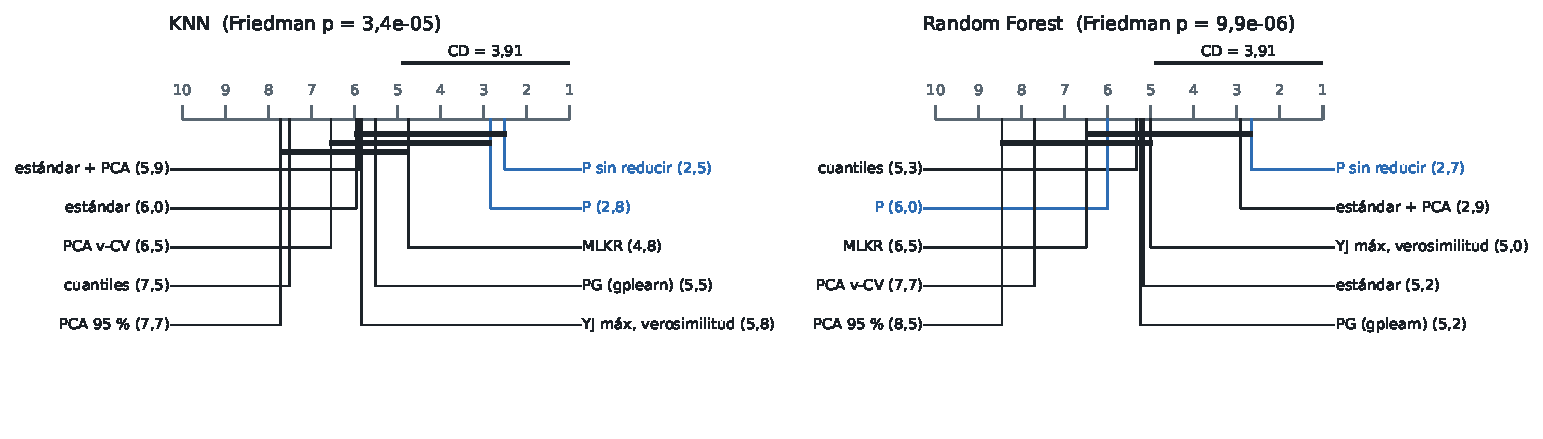
\includegraphics[width=\textwidth]{comparativa_cd2}
\caption{Diagramas de diferencia crítica. Eje: rango medio (a la derecha, mejor). Las barras gruesas unen métodos
que \emph{no} se distinguen. Con 11 métodos y 12 datasets la CD es grande: hacen falta más datasets para separar
los mejores.}
\end{figure}

\subsection{Modelos triviales y fijos}
Los cuatro modelos se usan con parámetros por defecto (KNN con $k=5$, RF con 100 árboles). El enunciado fija $M$: si
ajustáramos sus hiperparámetros estaríamos cambiando el modelo, no los datos, y no se podría atribuir la mejora a la
transformación.

\subsection{Cómo queda el resultado principal}
\begin{table}[h]\centering\small\setlength{\tabcolsep}{4pt}
\caption{$e'/e$ (media geométrica de los 12 datasets); $p$ por dataset con Holm; última columna, frente a $X$
estandarizado.}
\begin{tabular}{@{}lcccccc@{}}\toprule
Modelo & estándar & $P$ sin sínt. & $P$ & Datasets & $p$ & vs.\ est.\\\midrule
\filasPrincipal\bottomrule
\end{tabular}
\end{table}
\begin{idea}
En media, $e'<e$ en los cuatro modelos. \textbf{Concluyente para KNN} (\cambioKNN, $p=$\pKNN). Para la regresión
lineal (\cambioRL) y RF (\cambioRF) la mejora es consistente (10 de 12 datasets) pero, con 12 datasets y Holm, no
significativa. Así hay que contarlo.
\end{idea}

%=====================================================================================================
\section{Conceptos de computación evolutiva aplicados a la búsqueda}\label{sec:evolutiva}
Los apuntes previos explican CMA-ES ``por dentro''. Aquí lo leemos con el vocabulario general de los algoritmos
evolutivos y lo comparamos con el AG propio que usamos como contraste.

\subsection{Representación y espacio de búsqueda}
Cada individuo es $\theta\in\mathbb R^{2n}$ (codificación real). Se trabaja en el cubo $[0,1]^{2n}$ y se reescala a
los límites reales ($\lambda_j\in[-2,2]$, $w_j\in[0,3]$) al evaluar, para que un solo tamaño de paso sirva para todos
los parámetros.

\subsection{Población inicial}
\begin{definicion}[Población inicial]
Conjunto de soluciones de partida. En un AG es una lista de individuos; en una estrategia evolutiva como CMA-ES es
una \emph{distribución} de la que se muestrea: $\mathcal N(m_0,\sigma_0^2I)$.
\end{definicion}
\begin{itemize}
\item $m_0=\theta_0$: todos los $\lambda_j=1$ y $w_j=1$, es decir, la estandarización.
\item $\sigma_0=0{,}2$: el 20\,\% del rango de cada parámetro.
\item Tamaño $\lambda=4+\lfloor3\ln D\rfloor$: \popMin--\popMax{} candidatos por generación en nuestros datasets.
\item AG de contraste: $\theta_0$ + 29 individuos uniformes (30 en total).
\end{itemize}
\textbf{¿Importa?} No: partir de una media aleatoria (\ctrlIniAleat), $\sigma_0=0{,}1$ (\ctrlSigmaBajo) o $0{,}4$
(\ctrlSigmaAlto), o doblar la población (\ctrlPobDoble) no cambia el error de forma significativa. CMA-ES es robusto
a su inicio. Mantenemos $m_0=\theta_0$ porque arranca en la línea base razonable, hace la búsqueda reproducible e
interpretable (solo se aleja de estandarizar si el fitness lo justifica) y no compromete el resultado.

\subsection{Selección y presión selectiva}
\begin{definicion}[Presión selectiva]
Cuánto favorece la selección a los mejores individuos. Alta presión: converge rápido pero puede estancarse
(pérdida de diversidad). Baja: explora más pero avanza despacio.
\end{definicion}
\textbf{AG (torneo de $k$):} se cogen $k$ individuos al azar y gana el mejor; más $k$, más presión. Usamos $k=3$.

\textbf{CMA-ES (truncamiento ponderado por rango):} de los $\lambda$ candidatos se quedan los $\mu=\lfloor\lambda/2\rfloor$
mejores, con pesos decrecientes $w_i\propto\ln\frac{\lambda+1}{2}-\ln i$. La presión la fijan $\mu/\lambda$ y los
pesos, y se resume en la \textbf{masa efectiva de selección} $\mu_{\mathrm{eff}}=1/\sum_iw_i^2$ (aquí
\muEffMin--\muEffMax): es como si se seleccionaran $\sim$4 padres ``completos''.

\begin{figure}[h]\centering
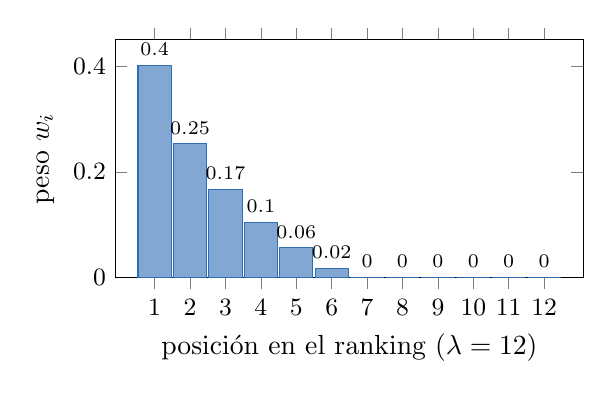
\begin{tikzpicture}
\begin{axis}[ybar, width=0.62\textwidth, height=4.6cm, bar width=12pt, ymin=0, ymax=0.45,
  xlabel={posición en el ranking ($\lambda=12$)}, ylabel={peso $w_i$}, xtick={1,...,12},
  ticklabel style={font=\small}, nodes near coords, nodes near coords style={font=\scriptsize},
  every node near coord/.append style={/pgf/number format/fixed, /pgf/number format/precision=2}]
\addplot[fill=azul!60, draw=azul] coordinates {(1,0.402) (2,0.253) (3,0.166) (4,0.104) (5,0.056) (6,0.017)
  (7,0) (8,0) (9,0) (10,0) (11,0) (12,0)};
\end{axis}
\end{tikzpicture}
\caption{Pesos de recombinación con $\lambda=12$: solo los 6 mejores contribuyen a la nueva media, el primero con un
40\,\%. $\mu_{\mathrm{eff}}=1/\sum w_i^2\approx3{,}73$.}
\end{figure}

\begin{nota}
Como la selección solo usa el \emph{orden}, CMA-ES es invariante a cualquier transformación monótona del fitness y
poco sensible a su ruido: una diferencia pequeña entre candidatos solo importa si cambia el orden.
\end{nota}

\subsection{Emparejamiento y recombinación}
\begin{definicion}[Recombinación (cruce)]
Combinar información de varios padres para generar descendencia.
\end{definicion}
\textbf{AG:} emparejamiento por parejas (dos torneos) y cruce \textbf{BLX-$\alpha$}: cada gen del hijo se toma
uniforme en el intervalo de los padres ampliado un $\alpha$ por cada lado,
$c_j=a_j+U(-\alpha,1+\alpha)\,(b_j-a_j)$, con $\alpha=0{,}3$.

\textbf{CMA-ES:} no hay parejas. La recombinación es \textbf{intermedia global ponderada}: la nueva media es
$m'=\sum_{i=1}^{\mu}w_i\,x_{i:\lambda}$, donde $x_{i:\lambda}$ es el $i$-ésimo mejor. Todos los seleccionados
contribuyen a la vez, lo que \emph{promedia el ruido} del fitness.

\subsection{Mutación}
\textbf{AG:} mutación gaussiana con probabilidad $1/D$ por gen y desviación del 10\,\% del rango.

\textbf{CMA-ES:} la ``mutación'' es el muestreo $x_k=m+\sigma y_k$, $y_k\sim\mathcal N(0,C)$, con $\sigma$ adaptado
por el camino evolutivo y $C$ por las actualizaciones de rango uno y rango $\mu$ (apuntes previos). La implementación
\texttt{pycma} usa además \emph{CMA activa}: los peores candidatos reciben pesos negativos en la actualización de $C$
para reducir la varianza en las direcciones malas.

\subsection{Inserción y reemplazo}
\begin{definicion}[Estrategias de reemplazo]
\textbf{$(\mu,\lambda)$} (coma): la siguiente generación sale \emph{solo} de los hijos; los padres se descartan.
\textbf{$(\mu+\lambda)$} (más): padres e hijos compiten juntos. \textbf{Elitismo}: el mejor siempre sobrevive.
\textbf{Generacional} frente a \textbf{estado estacionario}: se reemplaza toda la población de golpe o de uno en uno.
\end{definicion}
\begin{figure}[h]\centering
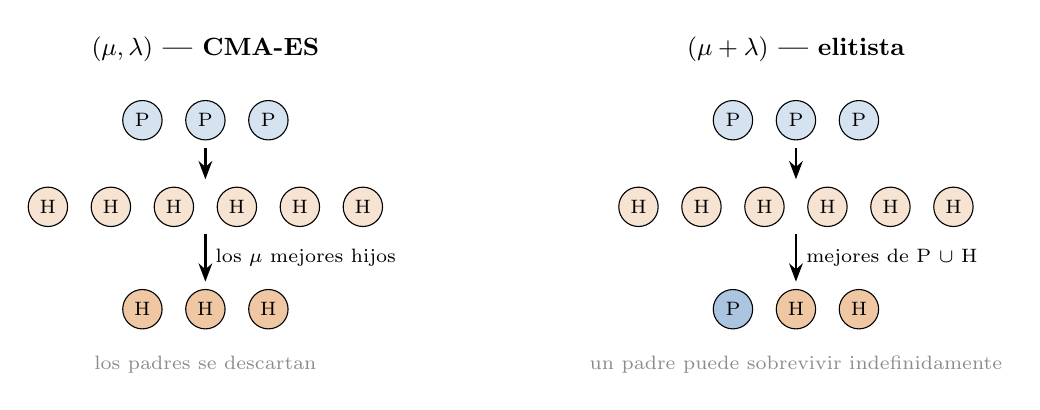
\begin{tikzpicture}[ind/.style={circle, draw, inner sep=2pt, minimum size=5mm, font=\scriptsize},
                    fl/.style={-{Stealth}, thick}]
\begin{scope}
\node[font=\small\bfseries] at (2,2.2) {$(\mu,\lambda)$ --- CMA-ES};
\foreach \i in {0,1,2} \node[ind, fill=azul!20] at (\i*0.8+1.2,1.3) {P};
\foreach \i in {0,...,5} \node[ind, fill=naranja!20] at (\i*0.8,0.2) {H};
\foreach \i in {0,1,2} \node[ind, fill=naranja!40] at (\i*0.8+1.2,-1.1) {H};
\draw[fl] (2,0.95) -- (2,0.55); \draw[fl] (2,-0.15) -- node[right, font=\scriptsize] {los $\mu$ mejores hijos} (2,-0.75);
\node[font=\scriptsize, gris] at (2,-1.8) {los padres se descartan};
\end{scope}
\begin{scope}[xshift=7.5cm]
\node[font=\small\bfseries] at (2,2.2) {$(\mu+\lambda)$ --- elitista};
\foreach \i in {0,1,2} \node[ind, fill=azul!20] at (\i*0.8+1.2,1.3) {P};
\foreach \i in {0,...,5} \node[ind, fill=naranja!20] at (\i*0.8,0.2) {H};
\node[ind, fill=azul!40] at (1.2,-1.1) {P}; \node[ind, fill=naranja!40] at (2.0,-1.1) {H};
\node[ind, fill=naranja!40] at (2.8,-1.1) {H};
\draw[fl] (2,0.95) -- (2,0.55); \draw[fl] (2,-0.15) -- node[right, font=\scriptsize] {mejores de P $\cup$ H} (2,-0.75);
\node[font=\scriptsize, gris] at (2,-1.8) {un padre puede sobrevivir indefinidamente};
\end{scope}
\end{tikzpicture}
\caption{Reemplazo coma frente a más.}
\end{figure}
\textbf{CMA-ES} usa $(\mu/\mu_w,\lambda)$: generacional y \textbf{no elitista}. Con un fitness ruidoso es una
ventaja: un candidato que salió bien ``por suerte'' en la validación cruzada no se queda para siempre. Aparte,
\texttt{pycma} guarda el mejor $\theta$ evaluado (un archivo externo), que es el que devolvemos.
\textbf{AG:} generacional con elitismo de 1 (el mejor pasa siempre).

\textbf{Restricciones.} Un candidato fuera de $[0,1]^D$ no se descarta: CMA-ES lo lleva al cubo con una
transformación suave (\emph{BoundTransform}); el AG lo recorta.

\subsection{Criterios de parada}
\begin{definicion}[Criterio de parada]
Condición que termina la búsqueda: presupuesto de evaluaciones o generaciones, estancamiento del fitness
(\texttt{tolfun}), de la solución (\texttt{tolx}), $\sigma$ demasiado pequeño, etc.
\end{definicion}
Usamos un \textbf{presupuesto de 1000 evaluaciones} (cada una es una validación cruzada completa), más las
tolerancias por defecto de \texttt{pycma}. Medido en los 12 datasets:
\begin{itemize}
\item Las \nParadaTotal{} búsquedas se detienen \textbf{por presupuesto} (\genMin--\genMax{} generaciones).
\item El mejor $\theta$ aparece de mediana en la evaluación \evalMejorMediana: la búsqueda \emph{seguía mejorando}.
\item $\sigma$ baja de $0{,}2$ a \sigmaFinMin--\sigmaFinMax: se está concentrando, pero no ha convergido del todo.
\item \texttt{pycma} termina la generación en curso: con $\lambda=12$ hace 1008 evaluaciones, no 1000.
\end{itemize}
\begin{cuidado}
Más presupuesto bajaría el fitness, pero en datos pequeños (diabetes) más fitness no es más validación: la búsqueda
aprende el ruido de los pliegues. El presupuesto es también una forma de regularización.
\end{cuidado}

\subsection{Resumen: CMA-ES frente al AG}
\begin{table}[h]\centering\small\setlength{\tabcolsep}{4pt}
\begin{tabular}{@{}p{2.4cm}p{6.6cm}p{4.6cm}@{}}\toprule
 & CMA-ES (método) & AG propio (contraste)\\\midrule
Inicio & distribución $\mathcal N(\theta_0,0{,}2^2I)$ & $\theta_0$ + 29 uniformes\\
Población & $\lambda=4+\lfloor3\ln D\rfloor$ (\popMin--\popMax) & 30\\
Selección & truncamiento por rango, $\mu=\lambda/2$, pesos logarítmicos & torneo de 3\\
Recombinación & intermedia ponderada de los $\mu$ (sin parejas) & BLX-$\alpha$ por parejas\\
Mutación & $\mathcal N(m,\sigma^2C)$; $\sigma$ y $C$ adaptativas; CMA activa & gaussiana, $p=1/D$\\
Reemplazo & $(\mu/\mu_w,\lambda)$, no elitista + mejor guardado & generacional + elitismo 1\\
Restricciones & transformación al cubo & recorte\\
Parada & 1000 evaluaciones (+ tolerancias) & 1000 evaluaciones\\\bottomrule
\end{tabular}
\end{table}

%=====================================================================================================
\section{Ablaciones de la búsqueda}\label{sec:ablacion}
Se cambia \emph{una sola decisión} cada vez, con la configuración final, en 24 particiones (12 datasets $\times$ 2).
\begin{table}[h]\centering\small\setlength{\tabcolsep}{6pt}
\caption{Cambio del MAE frente a $P$ ($>0$: peor que $P$; $^*$: $p<0{,}05$ por dataset con Holm).}
\begin{tabular}{@{}lccc@{}}\toprule
Variante & KNN & R.\ lineal & RF\\\midrule
\filasAblacion\bottomrule
\end{tabular}
\end{table}

\begin{definicion}[Información mutua]
$I(X_j;Y)$ mide cuánto reduce conocer $X_j$ la incertidumbre sobre $Y$, capturando también relaciones no lineales.
Usarla para fijar los pesos es un \emph{filtro}: puntúa cada atributo por separado, sin mirar el modelo ni las
interacciones.
\end{definicion}

\begin{itemize}
\item \textbf{Los pesos son la pieza clave}: sin ellos ($w=1$) KNN empeora \ctrlExp{} ($p=$\pCtrlExp). Sin
Yeo-Johnson ($\lambda=1$), \ctrlPesos{} en KNN y \ctrlPesosRL{} en RL, sin significación.
\item \textbf{La búsqueda importa}: la aleatoria con el mismo presupuesto es \ctrlAleat{} peor, y los pesos por
información mutua \ctrlMI: un filtro no sustituye a optimizar el error real.
\item \textbf{El inicio no importa} (sección anterior).
\item \textbf{El rango de $\lambda$ es poco crítico}: $[-1,1]$ \rangoUnoR, $[-4,4]$ \rangoCuatroR, $[-8,8]$ \rangoOchoR,
ninguno significativo. $[-2,2]$ no pierde frente a ninguna alternativa y evita el colapso numérico de los $\lambda$
extremos (el \mleFueraDos{} de los de máxima verosimilitud caen fuera).
\end{itemize}

\subsection{¿Importa el algoritmo?}
\begin{table}[h]\centering\small\setlength{\tabcolsep}{6pt}
\caption{Mismo $\theta$, fitness y presupuesto. Rango medio de fitness (1 = mejor) y cambio frente a $X$.}
\begin{tabular}{@{}lccc@{}}\toprule
Algoritmo & rango & KNN & R.\ lineal\\\midrule
\filasAlgoritmos\bottomrule
\end{tabular}
\end{table}
\begin{idea}
CMA-ES es el mejor en fitness, pero el AG, HS y BBO quedan a 1--2 puntos en validación; solo la búsqueda aleatoria es
claramente peor. \textbf{La búsqueda importa; el algoritmo concreto, bastante menos.} Es coherente con las críticas a
la proliferación de metaheurísticas ``de metáfora'' (Sörensen, 2015): lo que mueve el resultado es el problema y su
representación.
\end{idea}

%=====================================================================================================
\section{Coste computacional}\label{sec:coste}
Cada evaluación del fitness es una validación cruzada de KNN de 5 pliegues sobre $n_s\le2000$ filas. Calcular las
distancias de un pliegue cuesta $O\big((n_s/5)\cdot(4n_s/5)\cdot n\big)$, así que
\[
\text{coste de una búsqueda}\;\approx\;E\cdot O(n_s^2\,n),\qquad E=1000\text{ evaluaciones}.
\]
\begin{itemize}
\item Medido: \segMediana\,s de mediana por búsqueda (máximo \segMax\,s), $\sim$\msPorEval\,ms por evaluación, con
20 procesos en paralelo.
\item Alternativas (mediana): MLKR \segMLKR\,s, programación genética \segPG\,s, Yeo-Johnson por máxima verosimilitud
\segYJMV\,s.
\item Se paga una sola vez por dataset; aplicar la transformación después es inmediato. La síntesis duplica las
columnas, lo que encarece el entrenamiento de los árboles.
\end{itemize}

%=====================================================================================================
\section{¿Por qué la regresión lineal local queda fuera?}\label{sec:llr}
\begin{figure}[h]\centering
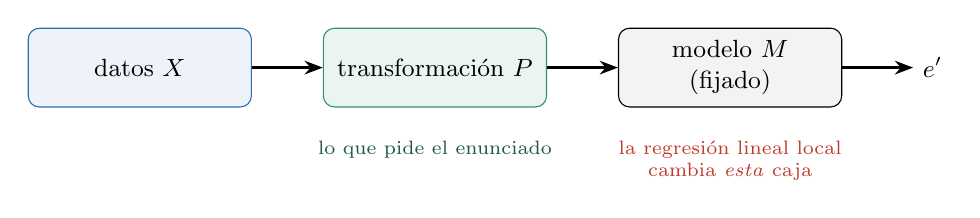
\begin{tikzpicture}[node distance=5mm and 9mm, caja/.style={draw, rounded corners, align=center, font=\small,
  minimum height=1cm, text width=2.6cm}, fl/.style={-{Stealth}, thick}]
\node[caja, fill=azul!8, draw=azul] (x) {datos $X$};
\node[caja, fill=verde!10, draw=verde, right=of x] (p) {transformación $P$};
\node[caja, fill=gris!10, right=of p] (m) {modelo $M$\\(fijado)};
\node[right=of m, font=\small] (e) {$e'$};
\draw[fl] (x)--(p); \draw[fl] (p)--(m); \draw[fl] (m)--(e);
\node[below=3mm of p, font=\scriptsize, verde!60!black, align=center] {lo que pide el enunciado};
\node[below=3mm of m, font=\scriptsize, rojo, align=center] {la regresión lineal local\\cambia \emph{esta} caja};
\end{tikzpicture}
\end{figure}
La regresión lineal local es una \emph{regla de predicción} (un modelo), no una transformación. No puede mejorar a
otro modelo trivial porque no cambia lo que ese modelo recibe. Lo que mostraba es que, si se pudiera elegir el
modelo, ``métrica aprendida + regresión lineal local'' sería el mejor predictor (0,64 del error de KNN original).
Pero el enunciado fija $M$, así que no cuenta para $e'<e$. Una variante legítima sería usarla como \emph{fitness}
en lugar de KNN, a cambio de búsquedas bastante más lentas: queda como trabajo futuro.

%=====================================================================================================
\section{Lo que nos criticarían y cómo se ha respondido}\label{sec:criticas}
\begin{table}[h]\centering\small\setlength{\tabcolsep}{4pt}
\begin{tabular}{@{}p{4.3cm}p{6.6cm}p{2.6cm}@{}}\toprule
Crítica & Respuesta & Estado\\\midrule
Faltan alternativas fuertes & 10 alternativas en las mismas particiones, incluidas MLKR y programación genética & hecho\\
``La mejora en árboles es solo PCA'' & Comprobado: es casi toda de añadir PCA; se dice así & hecho (aceptado)\\
Ablaciones con otra configuración & Repetidas con la configuración final (controles, inicio, rango, algoritmos) & hecho\\
Pseudo-replicación & Unidad = dataset; Wilcoxon + Holm; Friedman + Nemenyi & hecho\\
Modelos sin ajustar & Triviales por diseño: el enunciado fija $M$ & justificado\\
Coste & Medido y comparado & hecho\\
Rango de $\lambda$ con 500 evaluaciones & Repetido con 1000 & hecho\\
Figura de síntesis mezclada & Rehecha solo con confirmación & hecho\\
Pocos datasets, numéricos, pequeños & Ampliar a OpenML-CTR23 (35 problemas) & pendiente\\
Trabajo relacionado escaso & Búsqueda bibliográfica & pendiente\\
Paper desactualizado & Rehacer con estos resultados & pendiente\\\bottomrule
\end{tabular}
\end{table}

%=====================================================================================================
\section{Resumen para la defensa}
\begin{resultado}[Cinco frases]
\begin{enumerate}
\item Un único $X'$ reduce el error medio de cuatro modelos triviales; de forma concluyente en KNN (\cambioKNN) y
consistente pero no significativa con 12 datasets en regresión lineal y Random Forest.
\item La clave es diseñar $X'$ según qué es invariante para cada modelo: piezas que ayudan a una familia sin poder
perjudicar a las demás.
\item Frente a diez alternativas, $P$ tiene el mejor rango medio, pero en cada modelo alguna lo iguala (MLKR, PG, PCA
añadida).
\item La búsqueda importa (gana al azar y a los filtros); el algoritmo, el inicio y el rango de $\lambda$, poco.
\item Endurecer la evaluación cambió conclusiones: por eso todo lo reportado sale de particiones nuevas y de un
contraste por dataset.
\end{enumerate}
\end{resultado}

\begin{nota}[Ficheros]
\texttt{final/metodo.py} (programa $P$), \texttt{experimento\_final.py} (confirmación),
\texttt{experimento\_comparativa.py} (alternativas), \texttt{experimento\_busqueda.py} (varianza, controles, rango,
algoritmos, inicio), \texttt{experimento\_parada.py} (generaciones y parada), \texttt{analisis.py} (estadística,
figuras y cifras), \texttt{notebook\_final.ipynb}.
\end{nota}
\end{document}
